\begin{frame}{FastQ Format}

\begin{itemize}
\itemsep1pt\parskip0pt\parsep0pt
\item
  Standard Format for NGS data
\item
  Conversion can be done from \emph{sff}, \emph{fasta + qual}, \ldots{}
\item
  Extension of the Fasta format
\item
  Text-based formats (easy to use!)
\item
  If not compressed, it can be huge
\end{itemize}

~

\centering

\url{http://en.wikipedia.org/wiki/FASTQ_format}

\end{frame}

\begin{frame}{Quality measurements}

Base-calling \textbf{error probabilities} are reported by sequencers.

Usually in \textbf{Phred} (quality) score.

Usually coded by ASCII characters

\begin{block}{Phred score}

\[Q = -10 log_{10} P\]

\[P = 10^{\frac{-Q}{10}}\]

~

\url{http://en.wikipedia.org/wiki/Phred/_quality/_score\#Definition}

\end{block}

\end{frame}

\begin{frame}{NGS Data Preprocessing Steps}

\begin{itemize}
\item
  File parsing: convert to \textbf{fastq} format form \textbf{sff},
  \textbf{fasta} + \textbf{qual} \ldots{}
\item
  Split
  \href{http://www.illumina.com/technology/multiplexing_sequencing_assay.ilmn}{multiplex}
  samples.
\item
  Quality Control of the raw data.
\item
  Filtering and trimming reads by quality.
\item
  Adapter trimming
\item
  Quality Control of the trimmed and filtered reads
\end{itemize}

\end{frame}

\begin{frame}{Software}

\begin{itemize}
\itemsep1pt\parskip0pt\parsep0pt
\item
  \textbf{FastQC}:

  \begin{itemize}
  \itemsep1pt\parskip0pt\parsep0pt
  \item
    quality control
  \item
    some filtering \ldots{}
  \end{itemize}
\end{itemize}

~

\begin{itemize}
\itemsep1pt\parskip0pt\parsep0pt
\item
  \textbf{Cutadapt}:

  \begin{itemize}
  \itemsep1pt\parskip0pt\parsep0pt
  \item
    adapter trimming
  \item
    filter reads by length (short, long)
  \item
    filter reads by quality
  \end{itemize}
\end{itemize}

\end{frame}

\begin{frame}{Per Base Sequence Quality}

\begin{figure}[htbp]
\centering
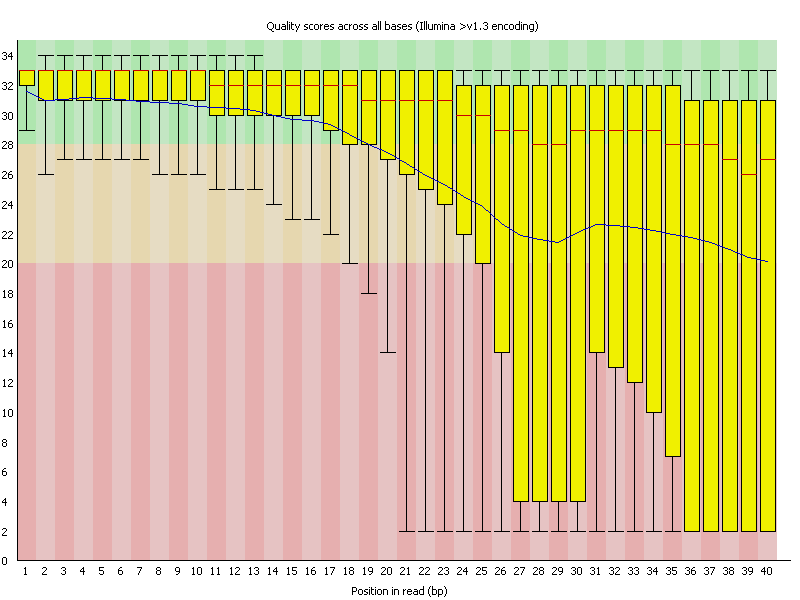
\includegraphics[width=\textwidth,height=0.8\textheight,keepaspectratio]{images/per_base_quality}
\end{figure}

\end{frame}

\begin{frame}{Per Sequence Quality}

\begin{figure}[htbp]
\centering
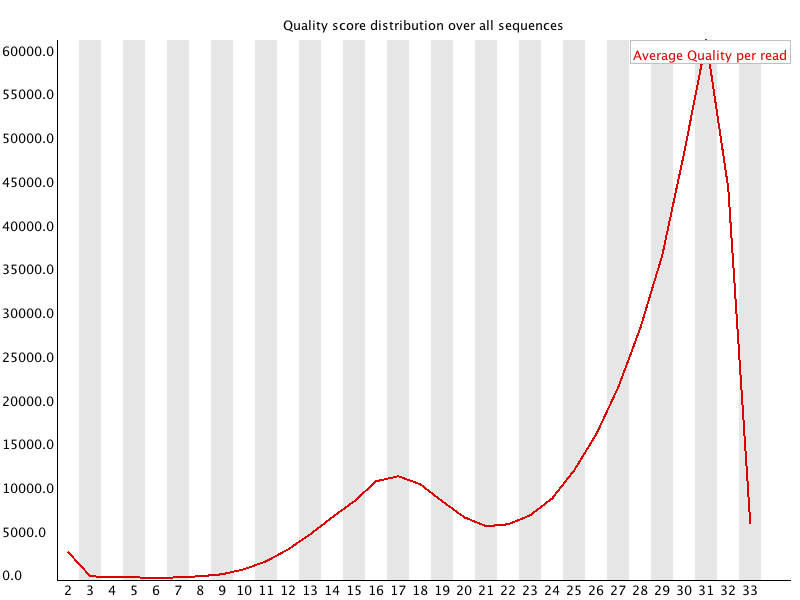
\includegraphics[width=\textwidth,height=0.8\textheight,keepaspectratio]{images/per_sequence_quality}
\end{figure}

\end{frame}

\begin{frame}{Per Base Sequence Content}

\begin{figure}[htbp]
\centering
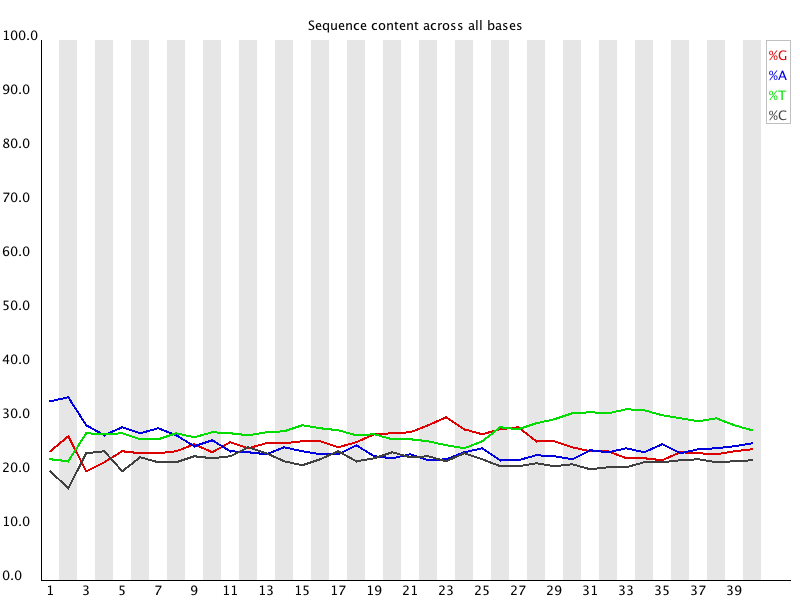
\includegraphics[width=\textwidth,height=0.8\textheight,keepaspectratio]{images/per_base_sequence_content}
\end{figure}

\end{frame}

\begin{frame}{Per Base GC Content}

\begin{figure}[htbp]
\centering
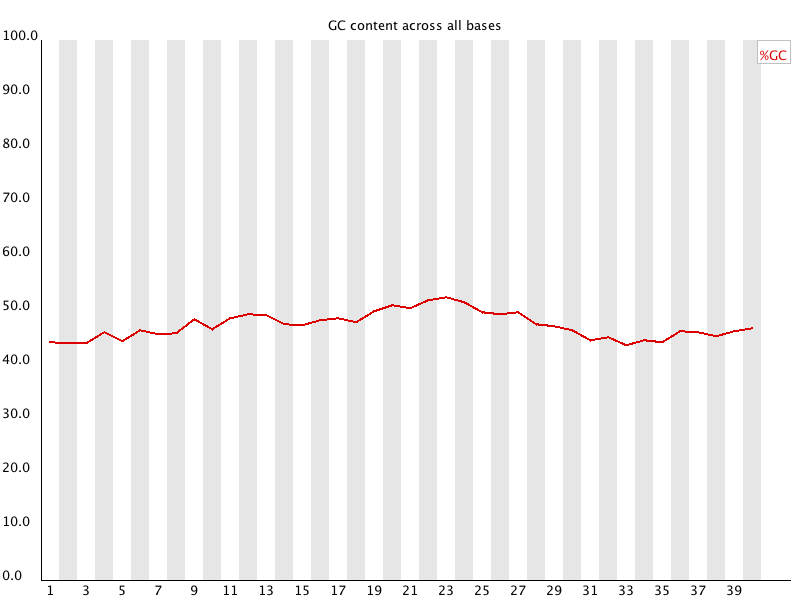
\includegraphics[width=\textwidth,height=0.8\textheight,keepaspectratio]{images/per_base_gc_content}
\end{figure}

\end{frame}

\begin{frame}{Per Sequence Nucleotide Content}

\begin{figure}[htbp]
\centering
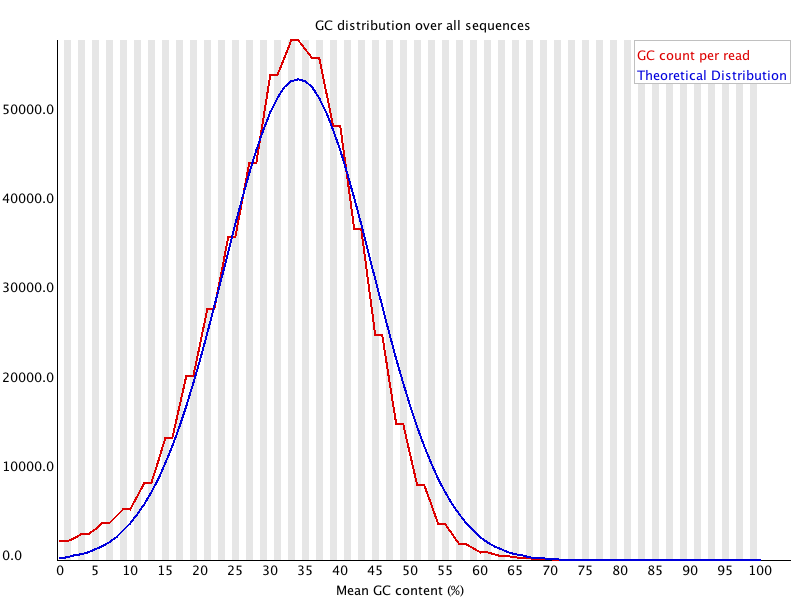
\includegraphics[width=\textwidth,height=0.8\textheight,keepaspectratio]{images/per_sequence_gc_content}
\end{figure}

\end{frame}

\begin{frame}{Per Base N Content}

\begin{figure}[htbp]
\centering
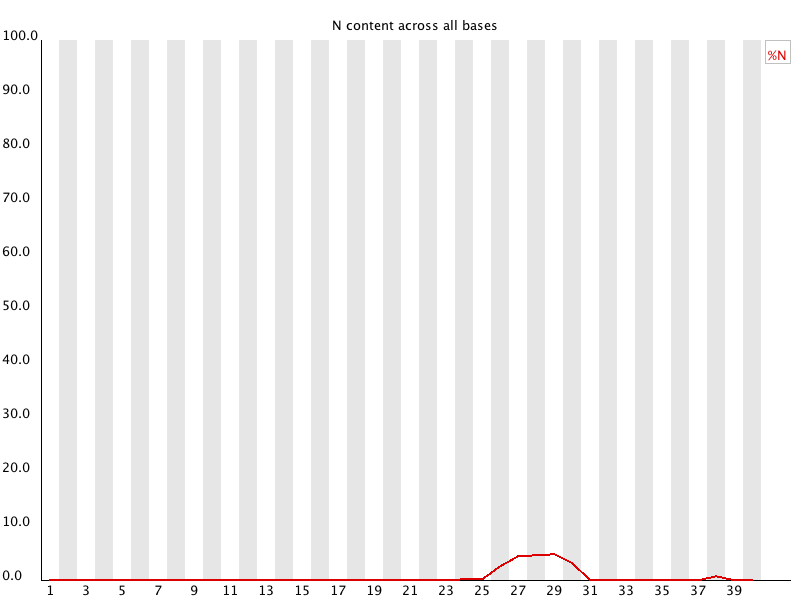
\includegraphics[width=\textwidth,height=0.8\textheight,keepaspectratio]{images/per_base_n_content}
\end{figure}

\end{frame}

\begin{frame}{Sequence Length Distribution}

\begin{figure}[htbp]
\centering
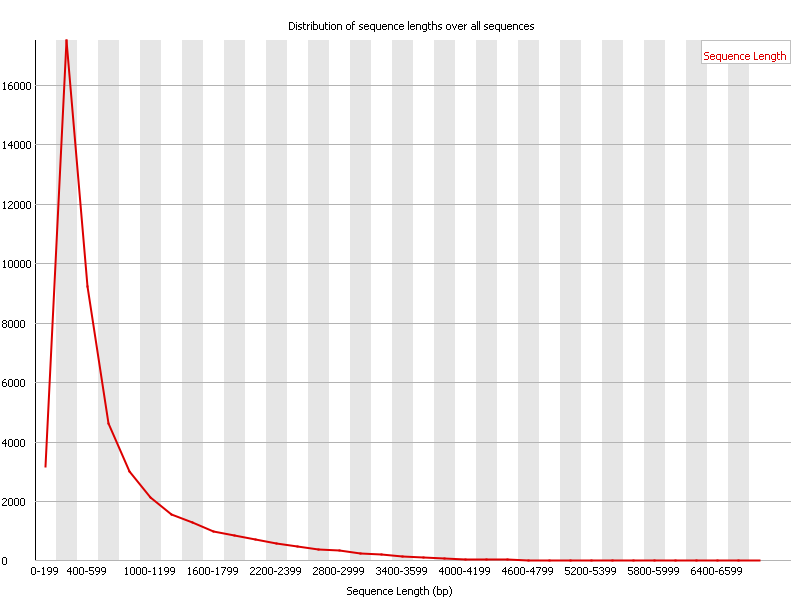
\includegraphics[width=\textwidth,height=0.8\textheight,keepaspectratio]{images/sequence_length_distribution}
\end{figure}

\end{frame}

\begin{frame}{Duplicate Sequences Distribution}

\begin{figure}[htbp]
\centering
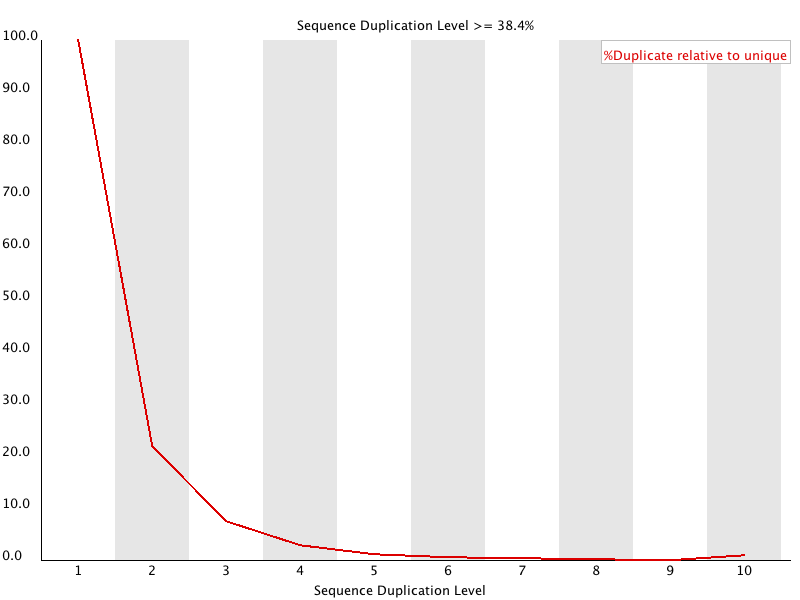
\includegraphics[width=\textwidth,height=0.8\textheight,keepaspectratio]{images/duplication_levels}
\end{figure}

\end{frame}

\begin{frame}{Overrepresented Kmers}

\begin{figure}[htbp]
\centering
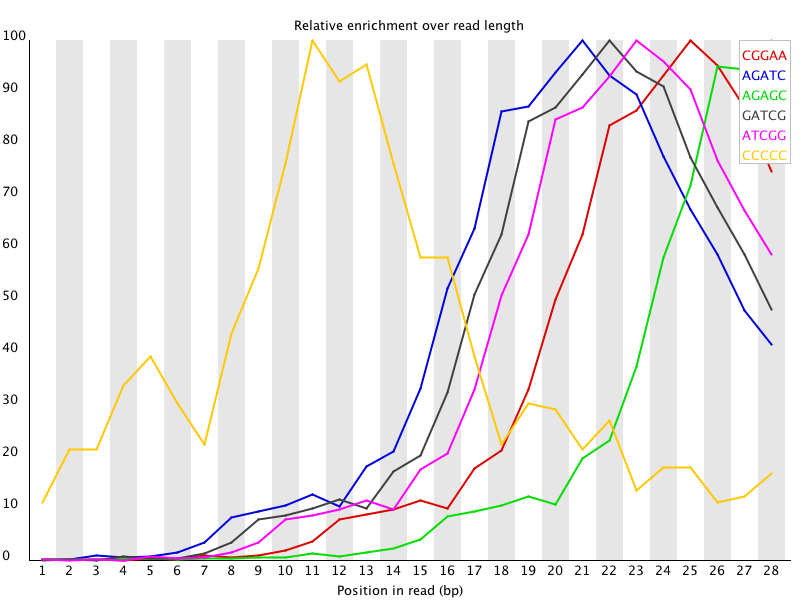
\includegraphics[width=\textwidth,height=0.8\textheight,keepaspectratio]{images/kmer_profiles}
\end{figure}

\end{frame}
